\chapter{Interfacing a Pushbutton}
\thispagestyle{empty}
\label{pushbutton}

\newcommand{\LocPushfig}{\Origin/user-code/push/figures}
\newcommand{\LocPushscicode}{\Origin/user-code/push/scilab}
\newcommand{\LocPushscibrief}[1]{{\tt
    \seqsplit{Origin/user-code/push/scilab/#1}}, 
see \fnrefp{fn:file-loc}}
\newcommand{\LocPushardcode}{\Origin/user-code/push/arduino}
\newcommand{\LocPushardbrief}[1]{{\tt
    \seqsplit{Origin/user-code/push/arduino/#1}}, 
see \fnrefp{fn:file-loc}}


%%%%%%%%%%%%%%python starts
\newcommand{\LocPushpycode}{\Origin/user-code/push/python}
\newcommand{\LocPushpybrief}[1]{{\tt
    \seqsplit{Origin/user-code/push/python/#1}}, 
see \fnrefp{fn:file-loc}}
%%%%%%%%%%%%%python ends

%%%%%%%%%%%%%%julia starts
\newcommand{\LocPushjuliacode}{\Origin/user-code/push/julia}
\newcommand{\LocPushjuliabrief}[1]{{\tt
    \seqsplit{Origin/user-code/push/julia/#1}}, 
see \fnrefp{fn:file-loc}}
%%%%%%%%%%%%%julia ends


%%%%%OpenModelica starts
\newcommand{\LocPushOpenModelicacode}{\Origin/user-code/push/OpenModelica}  %added for OpenModelica
\newcommand{\LocPushOpenModelicabrief}[1]{{\tt \seqsplit{%
    Origin/user-code/led/OpenModelica/#1}}, see \fnrefp{fn:file-loc}} % added for OpenModelica
%%%%%%OpenModelica Ends

A pushbutton is a simple switch which is used to connect or disconnect
a circuit. It is commonly available as a \emph{normally open} or
\emph{push to make} switch which implies that the contact is made upon
the push or depression of the switch. These switches are widely used
in calculators, computer keyboards, home appliances, push-button
telephones and basic mobile phones, etc. In this chapter, we shall
perform a few experiments to read the status of the pushbutton mounted
on the shield of the \arduino\ board. Advancing further, we shall
perform a few tasks depending on the status of the pushbutton. Digital
logic based status monitoring is a very basic and important task in
many industrial applications. This chapter will enable us to have a
smooth hands-on for such functionalities. 

\section{Preliminaries}
A pushbutton mounted on the shield is connected to the digital pin 12
of the \arduino\ board. The connection diagram for the pushbutton is
shown in \figref{fig:pushbuttonconn}. It has 2 pairs of
terminals. Each pair is electrically connected. When the pushbutton is
pressed all the terminals short to complete the circuit, thereby
allowing the flow of current through the switch. As you might expect,
there is a limit to the maximum current that could flow through a
pushbutton. This maximum current is also called the rated current and
is provided by the manufacturer in the datasheet.  

\begin{figure}
\centering
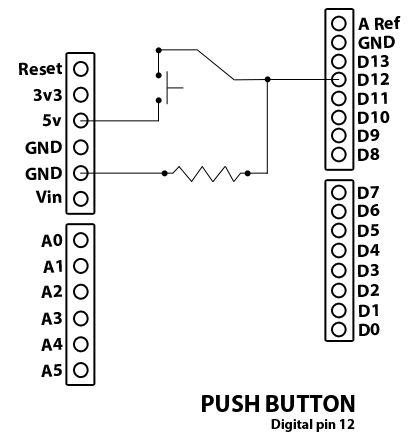
\includegraphics[width=\smfig]{\LocPushfig/pushbutton-conn.png}
\caption{Connection Diagram}
%\redcolor{connected on pin no. D12}}
\label{fig:pushbuttonconn}
\end{figure}

\section{Connecting a pushbutton with \arduino\ using a breadboard}
This section is useful for those who either don't have a shield or don't want to use the shield
for performing the experiments given in this chapter. 

To know more about the pushbutton, one should watch the Spoken Tutorials on Arduino as published on 
  {\tt https://spoken-tutorial.org/}. In case, you have a pushbutton and you want to try connecting it with \arduino\ on a breadboard, you should 
refer to the sixth tutorial titled Arduino with Tricolor LED and Push button on {\tt https://spoken-tutorial.org/}.
To know the connections, please refer to the figure \ref{fig:ard-pushbtn-bread}. The connections given in this 
figure can be used to read the status of a pushbutton. 

\begin{figure}
  \centering
  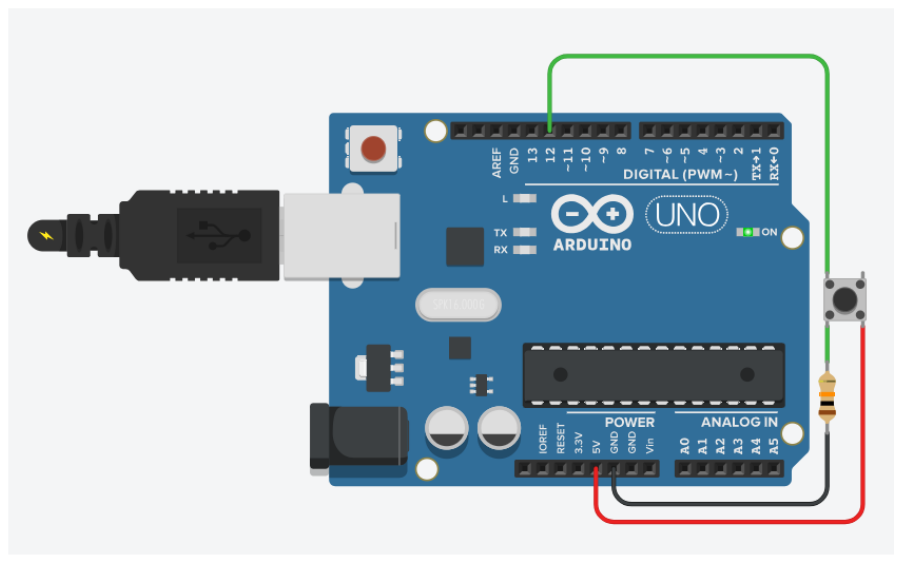
\includegraphics[width=\textwidth]{\LocPushfig/ard-pushbtn.png}
  \caption{Interfacing an RGB LED with Arduino Uno using a breadboard}
  %\redcolor{connected on pin no. D12}}
  \label{fig:ard-pushbtn-bread}
\end{figure}

\section{Reading the Pushbutton Status from the Arduino IDE}
\subsection{Reading the Pushbutton Status}
In this section, we shall learn commands to read the status of a
pushbutton through Arduino IDE. Later, we shall change the state of
the LED depending on the status of the pushbutton. 
\begin{enumerate}
\item In the first experiment, we shall simply read the status of the
  pushbutton. Recall that it is a normally open type of switch. So, in
  an unpressed state, the logic read will be ``0'', corresponding to
  0V. And, when the user presses the pushbutton, the reading would be
  ``1'', corresponding to 5V. The code for this experiment is given in
  \ardref{ard:push-100}. In the initialization part of the code, we
  assign the sensor pin to be read, 12 in this case, to a variable for
  ease. Next, we initialize the port for serial port communication at
  data rate of 9600 bits per second and declare the digital pin 12 as an input pin using the command {\tt pinMode}. After initialization, we start reading the status of the pushbutton using the following command:
  \lstinputlisting[firstline=5,lastline=5]
  {\LocPushardcode/push-button-status/push-button-status.ino}

  Note that the input argument to this command is the digital pin 12
  corresponding to the pin to which the pushbutton is connected.  After
  acquiring the values, we print them using,
  \lstinputlisting[firstline=8,lastline=8]
  {\LocPushardcode/push-button-status/push-button-status.ino} We
  repeat this read and print process 1000 times by putting the
  commands in a {\tt for} loop. At the same time, the user must press
  and release the pushbutton and observe the values printed on the
%  \redcolor{Serial monitor}.
serial monitor.

\item In the second experiment, we shall control the power given to an
  LED as per the status of the pushbutton. The code for this
  experiment is given in \ardref{ard:push-200}. This experiment can be
  taken as a step further to the previous one. We declare the LED pin
  to be controlled as an output pin by,
  \lstinputlisting[firstline=6,lastline=6]
  {\LocPushardcode/led-push-button/led-push-button.ino} Next, we read
  the potentiometer value from digital pin 12. If the value is ``1'',
  we turn on the LED at pin 9 else we turn it off. The
  condition check is performed using {\tt if else} statements. We run
  these commands for 1000 iterations.
\end{enumerate}

\subsection{Arduino Code}
\lstset{style=mystyle}
\label{sec:push-arduino-code}
\addtocontents{ard}{\protect\addvspace{\codclr}}

\begin{ardcode}
  \acaption{Read the status of the pushbutton and displaying on the
  serial monitor}{Read the status of the pushbutton and display it on
    the serial monitor.  Available at
    \LocPushardbrief{push-button-status/push-button-status.ino}.}
\label{ard:push-100}
\lstinputlisting{\LocPushardcode/push-button-status/push-button-status.ino}
\end{ardcode}

\begin{ardcode}
  \acaption{Turning the LED on or off depending on the pushbutton}
  {Turning the LED on or off depending on the pushbutton.  Available
    at \LocPushardbrief{led-push-button/led-push-button.ino}.}
\label{ard:push-200}
\lstinputlisting{\LocPushardcode/led-push-button/led-push-button.ino}
\end{ardcode}


\section{Reading the Pushbutton Status from Scilab}
\subsection{Reading the Pushbutton Status}
In this section, we shall perform the pushbutton operation using
Scilab-Arduino toolbox commands.
\begin{enumerate}
\item In the first experiment, we will read the pushbutton status in
  \scilab\ Console. The code for this experiment is given in
  \sciref{sci:push-100}. As explained earlier, we begin with serial
  port initialization. Then, using the command,
  \lstinputlisting[firstline=4,lastline=4]
  {\LocPushscicode/push-button-status.sce} we read the input of
  digital pin 12. Note that the middle terminal of the potentiometer
  is connected to this pin. The read value is displayed as a GUI using
  the command, \lstinputlisting[firstline=5,lastline=5]
  {\LocPushscicode/push-button-status.sce} where {\tt val} contains
  the potentiometer value acquired by the previous command. To
  encourage the user to have a good hands-on, we run these commands in
  a {\tt for} loop for 1000 iterations.

\item This experiment is an extension of the previous
  experiment. Here, we control the state of an LED as per the status
  of the pushbutton. In other words, digital output to an LED is
  decided by the digital input received from the pushbutton. The code
  for this experiment is given in \sciref{sci:push-200}. After reading
  the pushbutton status, we turn the LED on if the pushbutton is
  pressed, otherwise we turn it off. The lines,
  \lstinputlisting[firstline=5,lastline=9]
  {\LocPushscicode/led-push-button.sce} perform the condition check
  and corresponding LED state control operation.
\end{enumerate}

\subsection{Scilab Code}
\label{sec:push-scilab-code}
\addtocontents{cod}{\protect\addvspace{\codclr}}

\begin{scicode}
\ccaption{Read the status of the pushbutton and displaying on the
  serial monitor}{Read the status of the pushbutton and displaying on
    the serial monitor.  Available at
  \LocPushscibrief{push-button-status.sce}.}
\label{sci:push-100}
\lstinputlisting{\LocPushscicode/push-button-status.sce}
\end{scicode}

\begin{scicode}
\ccaption{Turning the LED on or off depending on the pushbutton}
  {Turning the LED on or off depending on the pushbutton.  Available at
  \LocPushscibrief{led-push-button.sce}.}
\label{sci:push-200}
\lstinputlisting{\LocPushscicode/led-push-button.sce}
\end{scicode}




\section{Accessing the Pushbutton from Xcos}
\label{sec:push-xcos}
In this section, we will see how to access the pushbutton from Scilab
Xcos.  We will carry out the same two experiments as in the previous
sections.  For each, will give the location of the zcos file and the
parameters to set.  The reader should go through the instructions
given in \secref{sec:xcos-start} before getting started.

\begin{enumerate}
\item First we will read the push button value and print it.  When the
  file required for this experiment is invoked, one gets the GUI as in
  \figref{fig:push-button-status}.  In the caption of this figure, one
  can see where to locate the file.

  As discussed in earlier chapters, we start with the initialization
  of the serial port. Next, using {\tt Digital Read} block, we read
  the status of potentiometer connected on digital pin 12. The read
  values are displayed.  When a user presses the pushbutton, change in
  the logic value from low to high can be observed.

  \begin{figure}
    \centering
    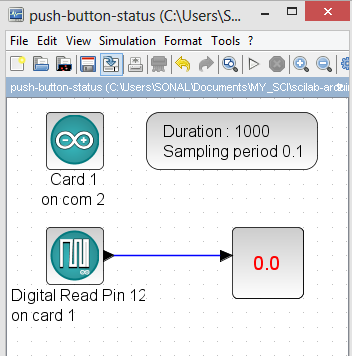
\includegraphics[width=\smfig]{\LocPushfig/push-button-status.PNG}
    \caption[Printing the push button status on the display block]
    {Printing the push button status on the display block.  This is
      what one sees when
        \LocPushscibrief{push-button-status.zcos}, is invoked.}
    \label{fig:push-button-status}
  \end{figure}

  We will next explain how to set the parameters for this simulation.
  To set value on any block, one needs to right click and open the
  {\tt Block Parameters} or double click.  The values for each block
  is tabulated in \tabref{tab:push-button-status}.  All other
  parameters are to be left unchanged.
  \begin{table}
    \centering
    \caption{Parameters to print the push button status on the display
      block} 
    \label{tab:push-button-status}
    \begin{tabular}{llc} \hline
      Name of the block & Parameter name & Value \\ \hline
      ARDUINO\_SETUP & Identifier of Arduino Card & 1 \\
      & Serial com port number & 2\portcmd \\ \hline
      TIME\_SAMPLE & Duration of acquisition(s) & 10 \\
      & Sampling period(s) & 0.1 \\ \hline
      DIGITAL\_READ\_SB & Digital pin & 12 \\
      & Arduino card number & 1 \\ \hline 
      AFFICH\_m & Block inherits(1) or not  (0) & 1 \\ \hline
    \end{tabular}
  \end{table}

\item In the second experiment, we take a step further and control the
  state of an LED in accordance with the status of the pushbutton. The
  Xcos implementation for this experiment is shown in
  \figref{fig:led-push-button}. Each time a user presses the
  pushbutton, the LED on digital pin 9 of the shield is switched
  on. If the shield is connected, the blue LED comes on.  When
  button is released, the LED is switched off. Here, we note that
  the digital logic level of the pin of the \arduino\ board connected
  to pushbutton changes only for the time the pushbutton is being
  pressed.

  \begin{figure}
    \centering
    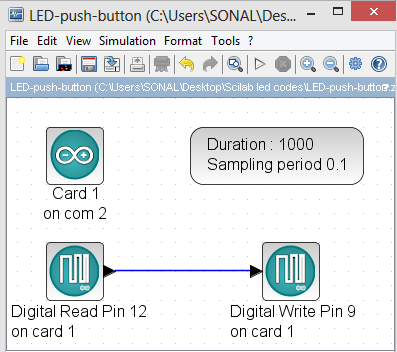
\includegraphics[width=\smfig]{\LocPushfig/led-push-button.PNG}
    \caption[Turning the LED on or off, depending on the pushbutton]
    {Turning the LED on or off, depending on the pushbutton.  This is
      what one sees when
        \LocPushscibrief{led-push-button.zcos}, is invoked.}
    \label{fig:led-push-button}
  \end{figure}

  We will next explain how to set the parameters for this simulation.
  To set value on any block, one needs to right click and open the
  {\tt Block Parameters} or double click.  The values for each block
  is tabulated in \tabref{tab:led-push-button}.  All other
  parameters are to be left unchanged.
  \begin{table}
    \centering
    \caption{Xcos parameters to turn the LED on through the pushbutton}
    \label{tab:led-push-button}
    \begin{tabular}{llc} \hline
      Name of the block & Parameter name & Value \\ \hline
      ARDUINO\_SETUP & Identifier of Arduino Card & 1 \\
      & Serial com port number & 2\portcmd \\ \hline
      TIME\_SAMPLE & Duration of acquisition(s) & 10 \\
      & Sampling period(s) & 0.1 \\ \hline
      DIGITAL\_READ\_SB & Digital pin & 12 \\
      & Arduino card number & 1 \\ \hline 
      DIGITAL\_WRITE\_SB & Digital pin & 9 \\
      & Card number & 1 \\ \hline
    \end{tabular}
  \end{table}
\end{enumerate}

\begin{exercise}
Let us carry out the following exercise:
\begin{enumerate}
\item In the above experiment, we controlled only one LED upon
  pushbutton press. Next, control multiple devices upon the pushbutton
  press. For example, upon press, turn on an LED and a motor and turn
  them off upon release.
\item Control several devices depending on the number of pushbutton
  press in a definite time span. For example, if the pushbutton is
  pressed once in time 't',say, turn on the LED. If it is pressed
  twice in time 't', turn on the motor. Here, you may want to consider
  the timing between two consecutive press.
\end{enumerate}
\end{exercise}

%%%%%%%%%%%%python description starts
\section{Reading the Pushbutton Status from Python}
\subsection{Reading the Pushbutton Status}
In this section, we shall perform the pushbutton operation using
Python-Arduino toolbox commands.
\begin{enumerate}
\item In the first experiment, we will read the pushbutton status in
  python Console. The code for this experiment is given in
  \pyref{py:push-100}. As explained earlier, we begin with serial
  port initialization. Then, using the command,
  \lstinputlisting[firstline=4,lastline=4]
  {\LocPushpycode/push-button-status.py} we read the input of
  digital pin 12. Note that the middle terminal of the potentiometer
  is connected to this pin. The read value is displayed as a GUI using
  the command, \lstinputlisting[firstline=5,lastline=5]
  {\LocPushpycode/push-button-status.py} where {\tt val} contains
  the potentiometer value acquired by the previous command. To
  encourage the user to have a good hands-on, we run these commands in
  a {\tt for} loop for 1000 iterations.

\item This experiment is an extension of the previous
  experiment. Here, we control the state of an LED as per the status
  of the pushbutton. In other words, digital output to an LED is
  decided by the digital input received from the pushbutton. The code
  for this experiment is given in \pyref{py:push-200}. After reading
  the pushbutton status, we turn the LED on if the pushbutton is
  pressed, otherwise we turn it off. The lines,
  \lstinputlisting[firstline=5,lastline=9]
  {\LocPushpycode/led-push-button.py} perform the condition check
  and corresponding LED state control operation.
\end{enumerate}

\subsection{Python Code}
\lstset{style=mystyle}
\label{sec:push-python-code}
\addtocontents{pyd}{\protect\addvspace{\codclr}}

\begin{pycode}
\pcaption{Read the status of the pushbutton and displaying on the
  serial monitor}{Read the status of the pushbutton and displaying on
    the serial monitor.  Available at
  \LocPushpybrief{push-button-status.py}.}
\label{py:push-100}
\lstinputlisting{\LocPushpycode/push-button-status.py}
\end{pycode}

\begin{pycode}
\pcaption{Turning the LED on or off depending on the pushbutton}
  {Turning the LED on or off depending on the pushbutton.  Available at
  \LocPushpybrief{led-push-button.py}.}
\label{py:push-200}
\lstinputlisting{\LocPushpycode/led-push-button.py}
\end{pycode}


\section{Reading the Pushbutton Status from Julia}
\subsection{Reading the Pushbutton Status} 
In this section, we shall perform the pushbutton operation using
Julia-Arduino toolbox commands.
\begin{enumerate}
\item In the first experiment, we will read the pushbutton status in
  Atoms-text-Editor\ Console. The code for this experiment is given in
  \juliaref{julia:push-100}. As explained earlier, we begin with serial
  port initialization by using the command,\lstinputlisting[firstline=7,lastline=7]
  {\LocPushjuliacode/push-button-status.jl} we read the input of
  digital pin 12. The status of the push button as '0' for off and
  '1' for on is dispalyed on the Atoms-Text-Editor console. To
  encourage the user to have a good hands-on, we run these commands in
  a {\tt for} loop for 100 iterations.

\item This experiment is an extension of the previous
  experiment. Here, we control the state of an LED as per the status
  of the pushbutton. In other words, digital output to an LED is
  decided by the digital input received from the pushbutton. The code
  for this experiment is given in \juliaref{julia:push-200}. After reading
  the pushbutton status, we turn the LED on if the pushbutton is
  pressed, otherwise we turn it off. The lines,
  \lstinputlisting[firstline=8,lastline=12]
  {\LocPushjuliacode/led-push-button.jl} perform the condition check
  and corresponding LED state control operation.
\end{enumerate}

\subsection{Julia Code}
\label{sec:push-julia-code}
\addtocontents{juliad}{\protect\addvspace{\codclr}}

\begin{juliacode}
\jcaption{Read the status of the pushbutton and displaying on the
  serial monitor}{Read the status of the pushbutton and displaying on
    the serial monitor.  Available at
  \LocPushjuliabrief{push-button-status.jl}.}
\label{julia:push-100}
\lstinputlisting{\LocPushjuliacode/push-button-status.jl}
\end{juliacode}

\begin{juliacode}
\jcaption{Turning the LED on or off depending on the pushbutton}
  {Turning the LED on or off depending on the pushbutton.  Available at
  \LocPushjuliabrief{led-push-button.jl}.}
\label{julia:push-200}
\lstinputlisting{\LocPushjuliacode/led-push-button.jl}
\end{juliacode}

\section{Reading the Pushbutton Status from OpenModelica}
\subsection{Reading the Pushbutton Status}
In this section, we shall perform the pushbutton operation using
OpenModelica-Arduino toolbox commands.
\begin{enumerate}
\item In the first experiment, we will read the pushbutton status in
  OpenModelica output Console. The code for this experiment is given in
  \OpenModelicaref{OpenModelica:push-100}. As explained earlier, we begin with serial
  port initialization. Then, using the command,
  \lstinputlisting[firstline=16,lastline=16]
  {\LocPushOpenModelicacode/push-button-status.mo} we read the input of
  digital pin 12. 
\item This experiment is same as previously done with Scilab-Arduino.
\end{enumerate}
%%%%%%%%%%%%OpenModelica decription ends

% \section{Do we need all these? \redcolor{Manas, please answer}}
% \subsection{Troubleshooting}
% You can check whether pushbutton is working correctly or not by
% checking the connections. If pushbutton is working correctly, all the
% 4 terminals show electrical short. You can check this with digital
% multimeter (DMM). When pushbutton is released two pairs of terminals are
% not connected to the other 2 terminals on the other side. However,
% each pair is still shorted. 


\subsection{OpenModelica Code}
\label{sec:led-OpenModelica-code}
\addtocontents{OpenModelicad}{\protect\addvspace{\codclr}}

\begin{OpenModelicacode}
\mcaption{Read the status of the pushbutton and displaying on the
  serial monitor}{Read the status of the pushbutton and displaying on
    the serial monitor.  Available at
  \LocPushOpenModelicabrief{push-button-status.mo}.}
\label{OpenModelica:push-100}
\lstinputlisting{\LocPushOpenModelicacode/push-button-status.mo}
\end{OpenModelicacode}

\begin{OpenModelicacode}
\mcaption{Turning the LED on or off depending on the pushbutton}
  {Turning the LED on or off depending on the pushbutton.  Available at
  \LocPushOpenModelicabrief{led-push-button.mo}.}
\label{OpenModelica:push-200}
\lstinputlisting{\LocPushOpenModelicacode/led-push-button.mo}
\end{OpenModelicacode}
%%%%%%%%%%%%%%%%%OpenModelica ends
